%!TEX root =../MemoriaTFM.tex
%El anterior comando permite compilar este documento llamando al documento raíz
\chapter{Descripción de la Técnica}\label{chp-02}
\epigraph{A good DevOps organization will free up developers to focus on doing what they do best: write software. }{Rob Steward, 2015\\Global Vicepresident at Verint-Systems}

\lettrine[lraise=-0.1, lines=2, loversize=0.2]{P}{ara} comprender el desarrollo del trabajo aquí presentado, tal y como se ha llevado a cabo, se debe conocer la situación en que éste se desarrolla, la tecnología de la que se dispone y los elementos existentes y necesarios, de una manera objetiva.

Es por esto, que el apartado actual está orientado a conocer las características de la realidad representada y a introducir las bases tecnológicas del presente \gls{TFM}, resaltando los conceptos más importantes.

\section{Metodología Ágil}

La tecnología actual avanza a una velocidad considerable, provocando a su paso la renovación de la gestión de proyectos informáticos, debiendo esta alcanzar la velocidad de los cambios ocasionados por esta aceleración. 

Así, la calidad, eficiencia, rapidez y flexibilidad en la entrega de un determinado producto se ha convertido en prioritaria, dando paso a la conocida como \textbf{Metodología Ágil}.

La Metodología Ágil envuelve un enfoque para la toma de decisiones en los proyectos software que plantean métodos de ingeniería del software basado en el desarrollo iterativo e incremental, donde los y  soluciones evolucionan con el tiempo según la necesidad del proyecto. Así el trabajo es realizado mediante la colaboración de equipos auto-organizados y multidisciplinarios, inmersos en un proceso compartido de toma de decisiones a corto plazo\cite{vera2014}.

La \autoref{agil} muestra el ciclo de vida en cada iteracción de esta metodología.

\begin{figure}[htbp]
	\centering
	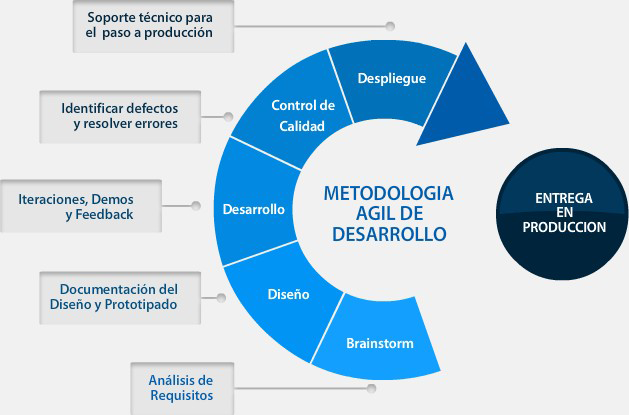
\includegraphics[width=1.0\linewidth]
	{tecnica/figuras/agil.png}
	\caption{CAMBIAR LA IMAGEN}
	\label{agil}
\end{figure}

El uso de procesos ágiles reporta los siguientes beneficios:

\begin{itemize}
	\item Flexibilidad en el proceso y las definiciones de los productos.
	\item Realimentación continua con el cliente.
	\item Iteracción constante del producto, que se va analizando a medida avanza.
	\item Calidad mejorada.
\end{itemize}


\section{Integración Continua \gls{IC} y Despliegue Continuo \gls{DC}}

Integración continua \gls{IC} es una práctica de desarrollo que requiere que los desarrolladores integren nuevos cambios en el código de la aplicación varias veces en un sólo día. Cada vez que esto ocurre, la inserción es verificada por una compilación automática, permitiendo a los equipos de trabajo implicados en el proceso detectar cualquier problema de forma temprana.

Integrando código regularmente los errores pueden ser detectados rápidamente y corregidos con más facilidad, debido a que al tratarse de un proceso frecuente la búsqueda del error va a quedar muy acotada.

El Despliegue Continuo \gls{DC} está estrechamente relacionado a la \gls{IC} y está referido a la liberación en los entornos de producción de la compañía de \gls{SW} que está continuamente siendo probado de manera automática.

Adoptar ambos conceptos (\gls{IC} y \gls{DC}) no solo reduce los riesgos y permite una localización temprana de fallos de código, sino que también permite aumentar la velocidad de trabajo con el \gls{SW}\cite{IC2017}.

\section{Ciclo de Desarrollo Seguro de software (\gls{SDLC})}

Un ciclo de Desarrollo Seguro de software (en inglés, Software Development Life Cycle \gls{SDLC}) es un marco de trabajo que define el proceso utilizado por las compañías a la hora de construir una aplicación desde sus inicios hasta el desmantelamiento de la misma. A lo largo de los últimos años,han surgido multitud de modelos para \gls{SDLC}, que han sido utilizados de diversas maneras acorde a las circunstancias de cada aplicación o empresa en general. Las fases comunes a todos estos modelos para el Ciclo de Desarrollo de software son las siguientes:

\begin{itemize}
	\item Requisitos y planificación.
	\item Arquitectura y diseño.
	\item Planificación de las pruebas.
	\item Desarrollo del código.
	\item Pruebas y resultados.
	\item Lanzamiento y mantenimiento.
\end{itemize}

Con esto, un proceso de implementación de seguridad en el proceso \gls{SDLC} garantizará que las actividades de seguridad, como las pruebas de penetración, la revisión del código y el análisis de la arquitectura, son parte integral del esfuerzo de desarrollo.

\section{Análisis estático}


\TODO{static analysis (static code analysis)\\Static analysis, also called static code analysis, is a method of computer program debugging that is done by examining the code without executing the program. The process provides an understanding of the code structure, and can help to ensure that the code adheres to industry standards. Automated tools can assist programmers and developers in carrying out static analysis. The process of scrutinizing code by visual inspection alone (by looking at a printout, for example), without the assistance of automated tools, is sometimes called program understanding or program comprehension.\\The principal advantageof  static analysis is the fact that it can reveal errors that do not manifest themselves until a disaster occurs weeks, months or years after release. Nevertheless, static analysis is only a first step in a comprehensive software quality-control regime. After static analysis has been done, dynamic analysis is often performed in an effort to uncover subtle defects or vulnerabilities. In computer terminology, static means fixed, while dynamic means capable of action and/or change. Dynamic analysis involves the testing and evaluation of a program based on execution. Static and dynamic analysis, considered together, are sometimes referred to as glass-box testing.}

\cite{rouse2017}

Análisis estático de software es un tipo de análisis de software que se realiza sin ejecutar el programa (el análisis realizado sobre los programas en ejecución se conoce como análisis dinámico de software).1​ En la mayoría de los casos, el análisis se realiza en alguna versión del código fuente y en otros casos se realiza en el código objeto. El término se aplica generalmente a los análisis realizados por una herramienta automática, el análisis realizado por un humano es llamado comprensión de programas (o entendimiento de programas) como también revisión de código.



\subsection{Ruby y NodeJS}

\TODO{YAML no e stá por ningún lado.}

Quizás a estas alturas no sea necesario hablar de estos lenguajes de programación... lo que si que daré será algunos datos que confirmen un poco por qué he empezado con estos...

\TODO{Breve presentación a la importancia de estos lenguajes de programación, comentando que lo que se ha hecho aquí es extensible a otros lenguajes, con otras herramientas similares.\\Concepto dependencias de código.}

Bundler is the de facto way of managing dependencies. It provides, among other things, a clear way of specifying required libraries and their versions, by keeping track of everything for you through Gemfile and (for applications) Gemfile.lock. Exactly the sort of information you’d need when checking for security vulnerabilities.

\subsection{De las dependencias del código}

\TODO{¿Qué es y cómo funciona?}

\subsection{De contenedores de imágenes}

\TODO{Quizás no son necesarios los subapartados... y simplemente baste con explicar elconcepto de análisis estático de algo genérico.}

https://www.linuxadictos.com/docker-i-que-es-conociendo-la-ballena.html

http://www.javiergarzas.com/2015/07/que-es-docker-sencillo.html

https://www.redeszone.net/2016/02/24/docker-funciona-la-virtualizacion-contenedores/


La nube es cada vez más grande, más potente, cuenta con más usuarios que hacen uso de ella al mismo tiempo y, además, permite la ejecución de aplicaciones cada vez más potentes, por lo que, para garantizar el correcto funcionamiento de esta, tanto en el presente como en el futuro, es necesario utilizar una plataforma que optimice los recursos lo mejor posible y, al mismo tiempo, sea lo más escalable posible con el fin de poder ampliar sus características de forma sencilla cuando sea necesario.

La nube es sinónimo de virtualización. Ejecutar un sistema operativo virtual por cada instancia de una aplicación es un proceso muy pesado y poco optimizado, a la vez que lento. Por ello, la comunidad Linux ha trabajado en el concepto de contenedores, una nueva forma de optimizar recursos creando pequeños espacios virtuales de las aplicaciones necesarias cargando solo el núcleo de la aplicación y las dependencias, pero funcionando siempre sobre un único kernel, o sistema operativo. (Esquema de esta WEB)

\section{Trabajos relacionados}

\endinput